\documentclass[11pt,compress,t,notes=noshow, xcolor=table]{beamer}
\usepackage[]{graphicx}\usepackage[]{color}
% maxwidth is the original width if it is less than linewidth
% otherwise use linewidth (to make sure the graphics do not exceed the margin)
\makeatletter
\def\maxwidth{ %
  \ifdim\Gin@nat@width>\linewidth
    \linewidth
  \else
    \Gin@nat@width
  \fi
}
\makeatother

\definecolor{fgcolor}{rgb}{0.345, 0.345, 0.345}
\newcommand{\hlnum}[1]{\textcolor[rgb]{0.686,0.059,0.569}{#1}}%
\newcommand{\hlstr}[1]{\textcolor[rgb]{0.192,0.494,0.8}{#1}}%
\newcommand{\hlcom}[1]{\textcolor[rgb]{0.678,0.584,0.686}{\textit{#1}}}%
\newcommand{\hlopt}[1]{\textcolor[rgb]{0,0,0}{#1}}%
\newcommand{\hlstd}[1]{\textcolor[rgb]{0.345,0.345,0.345}{#1}}%
\newcommand{\hlkwa}[1]{\textcolor[rgb]{0.161,0.373,0.58}{\textbf{#1}}}%
\newcommand{\hlkwb}[1]{\textcolor[rgb]{0.69,0.353,0.396}{#1}}%
\newcommand{\hlkwc}[1]{\textcolor[rgb]{0.333,0.667,0.333}{#1}}%
\newcommand{\hlkwd}[1]{\textcolor[rgb]{0.737,0.353,0.396}{\textbf{#1}}}%
\let\hlipl\hlkwb

\usepackage{framed}
\makeatletter
\newenvironment{kframe}{%
 \def\at@end@of@kframe{}%
 \ifinner\ifhmode%
  \def\at@end@of@kframe{\end{minipage}}%
  \begin{minipage}{\columnwidth}%
 \fi\fi%
 \def\FrameCommand##1{\hskip\@totalleftmargin \hskip-\fboxsep
 \colorbox{shadecolor}{##1}\hskip-\fboxsep
     % There is no \\@totalrightmargin, so:
     \hskip-\linewidth \hskip-\@totalleftmargin \hskip\columnwidth}%
 \MakeFramed {\advance\hsize-\width
   \@totalleftmargin\z@ \linewidth\hsize
   \@setminipage}}%
 {\par\unskip\endMakeFramed%
 \at@end@of@kframe}
\makeatother

\definecolor{shadecolor}{rgb}{.97, .97, .97}
\definecolor{messagecolor}{rgb}{0, 0, 0}
\definecolor{warningcolor}{rgb}{1, 0, 1}
\definecolor{errorcolor}{rgb}{1, 0, 0}
\newenvironment{knitrout}{}{} % an empty environment to be redefined in TeX

\usepackage{alltt}
\newcommand{\SweaveOpts}[1]{}  % do not interfere with LaTeX
\newcommand{\SweaveInput}[1]{} % because they are not real TeX commands
\newcommand{\Sexpr}[1]{}       % will only be parsed by R
\newcommand{\xmark}{\ding{55}}%


\usepackage[english]{babel}
\usepackage[utf8]{inputenc}

\usepackage{dsfont}
\usepackage{verbatim}
\usepackage{amsmath}
\usepackage{amsfonts}
\usepackage{amssymb}
\usepackage{bm}
\usepackage{csquotes}
\usepackage{multirow}
\usepackage{longtable}
\usepackage{booktabs}
\usepackage{enumerate}
\usepackage[absolute,overlay]{textpos}
\usepackage{psfrag}
\usepackage{algorithm}
\usepackage{algpseudocode}
\usepackage{eqnarray}
\usepackage{arydshln}
\usepackage{tabularx}
\usepackage{placeins}
\usepackage{tikz}
\usepackage{setspace}
\usepackage{colortbl}
\usepackage{mathtools}
\usepackage{wrapfig}
\usepackage{bm}
\usepackage{amsmath}
\usepackage{pifont}
\usepackage[round]{natbib}
\usepackage{hyperref}

\usetikzlibrary{shapes,arrows,automata,positioning,calc,chains,trees, shadows}
\tikzset{
  %Define standard arrow tip
  >=stealth',
  %Define style for boxes
  punkt/.style={
    rectangle,
    rounded corners,
    draw=black, very thick,
    text width=6.5em,
    minimum height=2em,
    text centered},
  % Define arrow style
  pil/.style={
    ->,
    thick,
    shorten <=2pt,
    shorten >=2pt,}
}

\usepackage{subfig}

% Defines macros and environments
\usepackage{../../style/lmu-lecture}


\let\code=\texttt
\let\proglang=\textsf

\setkeys{Gin}{width=0.9\textwidth}

\setbeamertemplate{frametitle}{\expandafter\uppercase\expandafter\insertframetitle}

% basic latex stuff
\newcommand{\pkg}[1]{{\fontseries{b}\selectfont #1}} % fontstyle for R packages

% Often used in exercise Rnw files, still relevant?
\newcommand{\lz}{\vspace{0.5cm}} % vertical space
\newcommand{\dlz}{\vspace{1cm}}  % double vertical space

% Unused and about to be deleted
\newcommand{\oneliner}[1] % Oneliner for important statements
{\begin{block}{}\begin{center}\begin{Large}#1\end{Large}\end{center}\end{block}}


%--------------------%
%  New environments  %
%--------------------%

 % Frame with breaks and verbatim // this is used very often
\newenvironment{vbframe}
{
\begin{frame}[containsverbatim,allowframebreaks]
}
{
\end{frame}
}

% Frame with verbatim without breaks (to avoid numbering one slided frames)
% This is not used anywhere but I can see it being useful
\newenvironment{vframe}
{
\begin{frame}[containsverbatim]
}
{
\end{frame}
}

% Itemize block
\newenvironment{blocki}[1]
{
\begin{block}{#1}\begin{itemize}
}
{
\end{itemize}\end{block}
}

%--------------%
%  Citebutton  %
%--------------%
% Example usage (from slides-cart-discussion.tex)
% \citebutton{Breiman, 1984}{https://www.taylorfrancis.com/books/mono/10.1201/9781315139470/classification-regression-trees-leo-breiman}
\newcommand{\citebutton}[2]{%
\NoCaseChange{\resizebox{!}{9pt}{\protect\beamergotobutton{\href{#2}{#1}}}}%
}

% textcolor that works in mathmode
% https://tex.stackexchange.com/a/261480
% Used e.g. in forests/slides-forests-bagging.tex
% [...] \textcolor{blue}{\tfrac{1}{M}\sum^M_{m} [...]
\makeatletter
\renewcommand*{\@textcolor}[3]{%
  \protect\leavevmode
  \begingroup
    \color#1{#2}#3%
  \endgroup
}
\makeatother







%\newcommand{\titlefigure}{} %MISSING!
\newcommand{\learninggoals}{
  \item XXXXXXXXXXXXXX
  \item XXXXXXXXX
}




\title{Introduction to Machine Learning}
% \author{Bernd Bischl, Christoph Molnar, Daniel Schalk, Fabian Scheipl}
\institute{\href{https://compstat-lmu.github.io/lecture_i2ml/}{compstat-lmu.github.io/lecture\_i2ml}}
\date{}




\begin{document}

\lecturechapter{Evaluation: Learning Curves}
\lecture{Introduction to Machine Learning}

\begin{vbframe}{Learning Curves}

\begin{itemize}
\item The \textit{Learning Curve} compares the performance of a model on training and test data over a varying number of training instances.\\
$\rightarrow$ How fast can learner learn the given relationship in the data?
\item Learning usually fast in the beginning %and saturate after data becomes larger an larger
% \item We should generally see performance improve as the number of training points increases When we separate training and testing sets and graph them individually
% \item We can get an idea of how well the model can generalize to new data
\item Visualizes when a learner has learned as much as it can:
\begin{itemize}
\item when performance on training and test set reach a plateau.
\item when gap between training and test error remains the same.
\end{itemize}
\end{itemize}





\begin{knitrout}\scriptsize
\definecolor{shadecolor}{rgb}{0.969, 0.969, 0.969}\color{fgcolor}

{\centering 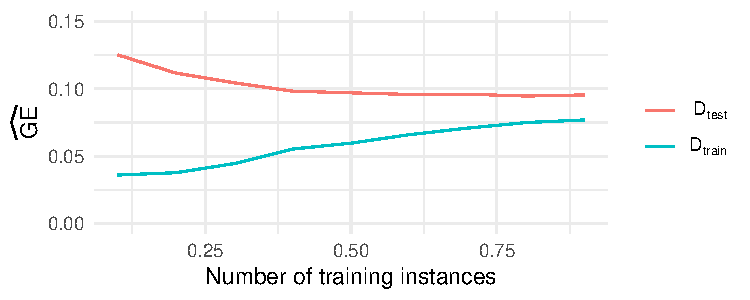
\includegraphics[width=0.9\textwidth]{figure/eval_learn_curves_1} 

}



\end{knitrout}

\framebreak

An ideal learning curve looks like:

\begin{knitrout}\scriptsize
\definecolor{shadecolor}{rgb}{0.969, 0.969, 0.969}\color{fgcolor}

{\centering 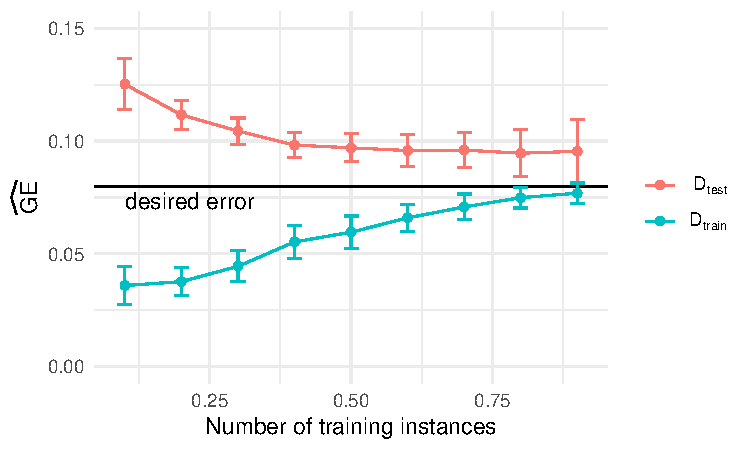
\includegraphics[width=0.95\textwidth]{figure/eval_learn_curves_2} 

}



\end{knitrout}


\framebreak

In general, there are two reasons for a bad looking learning curve:

\begin{enumerate}
\item High bias in model / underfitting
\begin{itemize}
\item training and test errors converge at a high value.
\item model can't learn underlying relationship and has high systematic errors, no matter how big the training set.
\item poor fit, which also translates into high test error.
\end{itemize}

\begin{knitrout}\scriptsize
\definecolor{shadecolor}{rgb}{0.969, 0.969, 0.969}\color{fgcolor}

{\centering 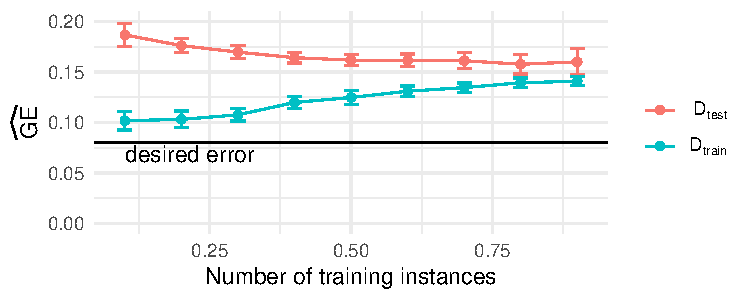
\includegraphics[width=0.95\textwidth]{figure/eval_learn_curves_3} 

}



\end{knitrout}

\framebreak

\item High variance in model / Overfitting
\begin{itemize}
\item large gap between training and test errors.
\item model requires more training data to improve.
\item model has a poor fit and does not generalize well.
%\item Can simplify the model with fewer or less complex features
\end{itemize}

\begin{knitrout}\scriptsize
\definecolor{shadecolor}{rgb}{0.969, 0.969, 0.969}\color{fgcolor}

{\centering 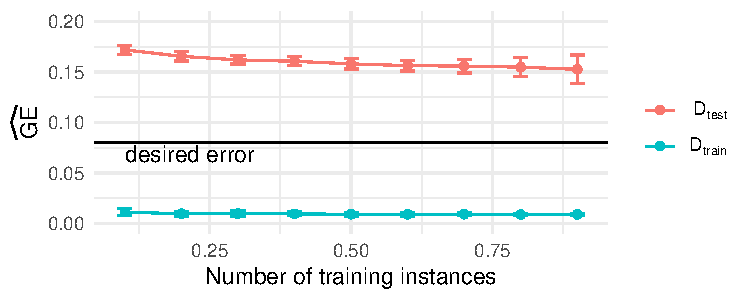
\includegraphics[width=0.95\textwidth]{figure/eval_learn_curves_4} 

}



\end{knitrout}
\end{enumerate}
\end{vbframe}

\endlecture

\end{document}
